\documentclass[11pt]{article}
\usepackage[a4paper,margin=1in]{geometry}
\usepackage{graphicx}
\usepackage{booktabs}
\usepackage{float}
\usepackage{amsmath}
\usepackage{hyperref}

\title{Behavior of the New Krotov Variants in the Two-Moons QML Optimization Benchmark}
\author{Codex experiment report}
\date{\today}

\begin{document}
\maketitle

\section*{Experimental setup}
The report analyzes the Krotov-family optimizers in the existing two-moons QML benchmark without changing the model or dataset pipeline. The setup uses 4 qubits, 3 trainable layers, 5 random seeds, and 100 outer iterations on the same train/test split convention as the original benchmark. The main comparison uses:
\begin{itemize}
\item \texttt{krotov\_online}: the preserved single-sample stale-adjoint update with constant step size $0.3$,
\item \texttt{krotov\_batch}: the new full-batch Krotov-inspired update with constant step size $0.3$.
\end{itemize}

The fair accounting axis is the propagation cost
\[
\text{cost units} = \text{sample forward passes} + \text{sample backward passes},
\]
which treats one single-sample forward propagation and one single-sample adjoint propagation as the primitive work units. Mean-loss evaluations and gradient-direction evaluations are logged separately in the raw JSON files, but the report uses cost units when interpreting optimization speed.

\section*{Main empirical findings}
\begin{enumerate}
\item The online Krotov baseline still shows the aggressive initial descent that motivated the original implementation. Averaged over seeds, its loss after the first optimization step is 0.382, compared with 0.702 for the full-batch variant.
\item The full-batch update is markedly smoother but substantially less aggressive at the baseline step size. Its mean final loss is 0.436 compared with 0.371 for the online variant.
\item The online method pays for its fast initial progress with persistent late-stage oscillation. Its mean tail loss standard deviation over the last 20 logged points is 0.028, versus 0.004 for the batch variant.
\item The batch update is strongly step-size limited rather than obviously broken. Across the sweep, the best mean final loss comes from \texttt{batch, lr=1.0}, which reaches 0.365. This is materially better than the baseline batch setting and indicates that the default batch step size was too conservative for this problem.
\end{enumerate}

\section*{Quantitative comparison of the main variants}
\begin{table}[H]
\centering
\begin{tabular}{lcccccc}
\toprule
Variant & Final loss & Final test acc. & Loss @ step 1 & Loss @ step 10 & Tail std. & Mean tail update norm \\
\midrule
online, lr=0.3 & 0.371 $\pm$ 0.034 & 0.856 $\pm$ 0.040 & 0.382 & 0.345 & 0.028 & 1.510 \\
batch, lr=0.3 & 0.436 $\pm$ 0.048 & 0.867 $\pm$ 0.018 & 0.702 & 0.629 & 0.004 & 0.014 \\
\bottomrule
\end{tabular}
\caption{Mean behavior of the main Krotov variants over the configured seeds. Tail statistics are computed from the last 20 logged optimization points.}
\end{table}

The table makes the central contrast explicit. The online variant is a high-gain optimizer: it descends quickly, reaches the lower mean final loss in the baseline comparison, and keeps relatively large updates even late in the run. The batch variant is much more regularized by construction because it averages the gate-wise contributions over the whole dataset before applying an update. That removes sample-order noise and the stale-adjoint inconsistency across successive samples, but it also suppresses the large coordinated moves that made the online rule effective at the beginning of training.

\begin{figure}[H]
\centering
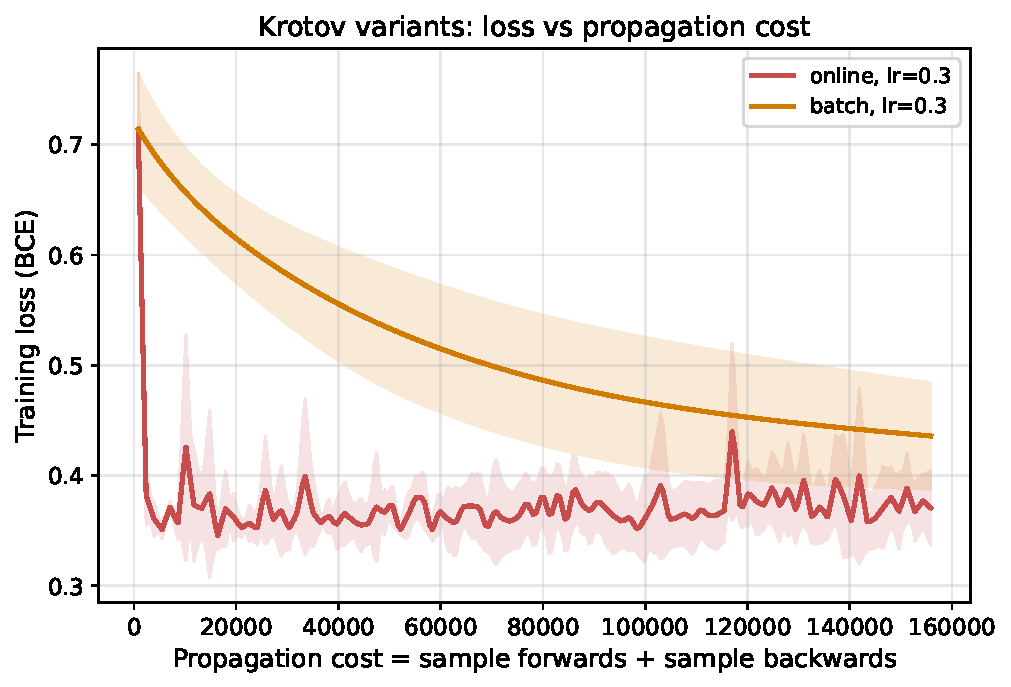
\includegraphics[width=0.8\linewidth]{figures/krotov_loss_vs_cost.pdf}
\caption{Training loss versus the fair propagation-cost metric for the main Krotov variants.}
\end{figure}

\begin{figure}[H]
\centering
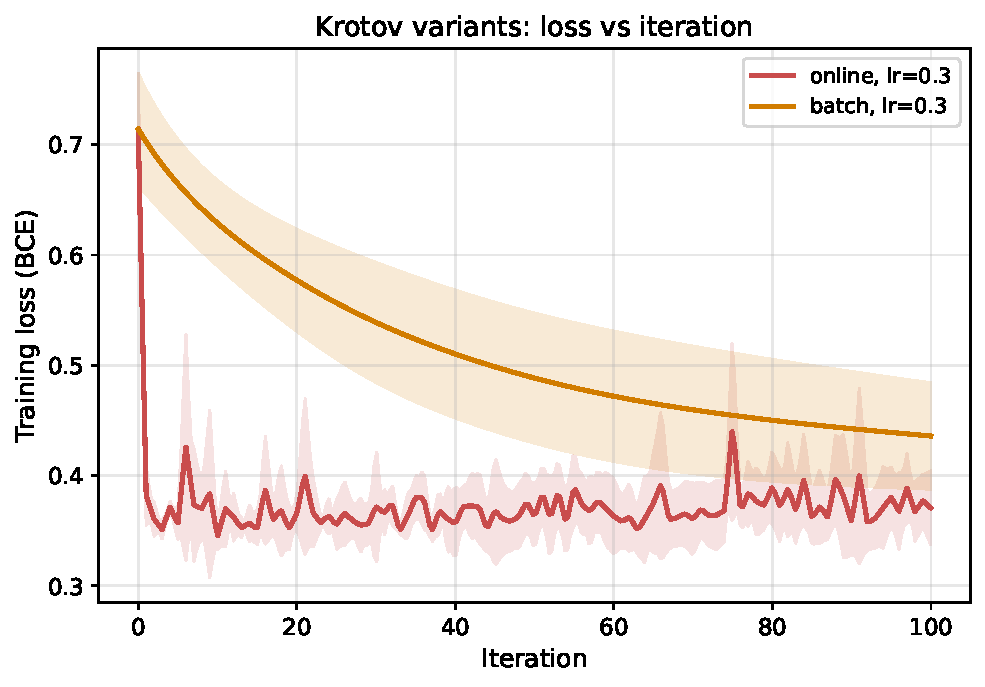
\includegraphics[width=0.8\linewidth]{figures/krotov_loss_vs_iteration.pdf}
\caption{Training loss versus iteration for the main Krotov variants.}
\end{figure}

\begin{figure}[H]
\centering
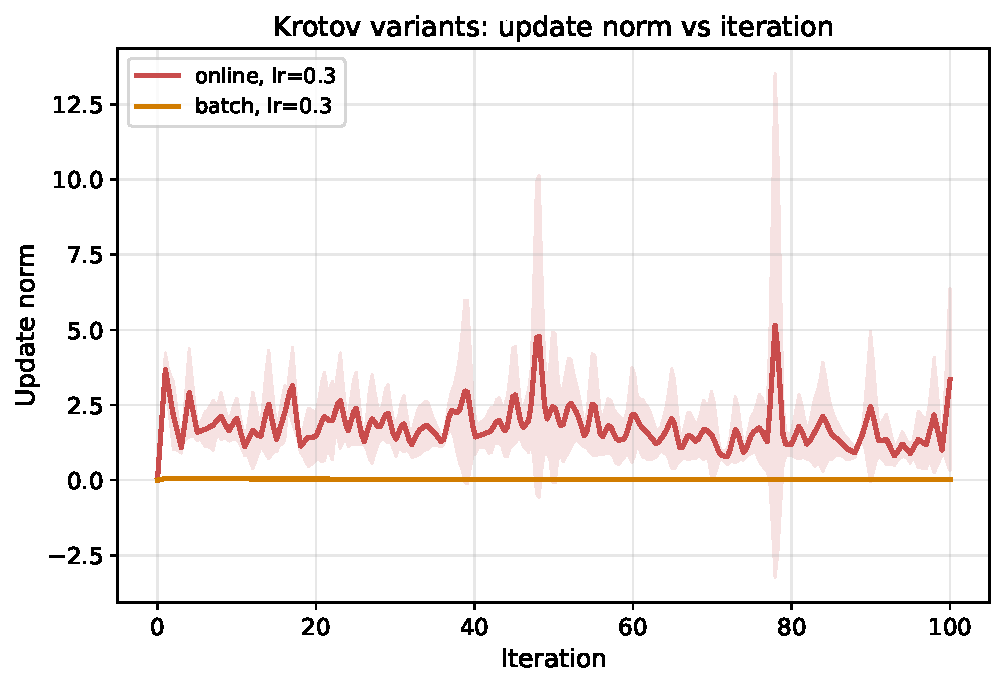
\includegraphics[width=0.8\linewidth]{figures/krotov_update_norm_vs_iteration.pdf}
\caption{Update norms reveal that the online rule keeps moving aggressively while the batch rule contracts to much smaller parameter changes.}
\end{figure}

\begin{figure}[H]
\centering
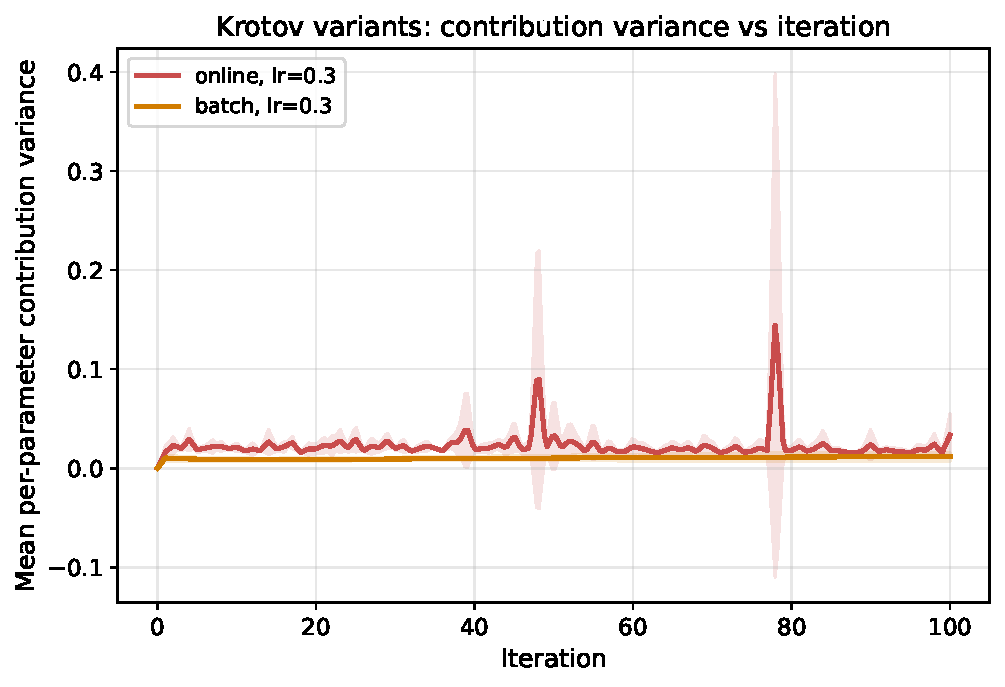
\includegraphics[width=0.8\linewidth]{figures/krotov_contribution_variance.pdf}
\caption{Per-parameter contribution variance. The online rule sees much noisier per-sample directions, which helps explain both the fast initial drop and the later oscillation.}
\end{figure}

\section*{Interpretation of the optimization dynamics}
The new diagnostics support a fairly specific interpretation of the Krotov behavior.

First, the online optimizer's rapid initial improvement is real under fair accounting. The loss decreases sharply in both the loss-versus-cost and loss-versus-iteration views. This means that the earlier observation was not an artifact of the old function-evaluation counter. The online rule is genuinely capable of finding a useful direction very quickly on this task.

Second, the same mechanism that makes the online method aggressive also makes it unstable. Each update is built from one sample at a time, and the backward co-states are computed before the subsequent gate-wise parameter changes. As a result, the method keeps taking relatively large, sample-specific steps even after it reaches a reasonably good decision boundary. The elevated contribution variance and tail update norms are consistent with exactly this picture.

Third, the full-batch variant behaves more like deterministic gradient descent in the gate-local coordinates. It aligns the update with the true benchmark objective, because the gate-wise contributions are averaged over the full training loss before a single parameter update is applied. This removes stale-adjoint accumulation across samples and collapses the sample-order noise, but it also means the update magnitude must be tuned more carefully. At the baseline step size of $0.3$, the batch method is simply too conservative.

\section*{Learning-rate sweep and what it implies}
\begin{table}[H]
\centering
\begin{tabular}{lccc}
\toprule
Batch variant & Final loss & Success rate (final loss $\leq 0.4$) & Mean cost to threshold \\
\midrule
batch, lr=0.3 & 0.436 $\pm$ 0.048 & 0.20 & 98500 \\
batch, lr=1.0 & 0.365 $\pm$ 0.036 & 0.80 & 64788 \\
batch, lr=0.1 & 0.528 $\pm$ 0.056 & 0.00 & nan \\
batch, lr=0.05 & 0.592 $\pm$ 0.043 & 0.00 & nan \\
batch, lr=0.02 & 0.652 $\pm$ 0.039 & 0.00 & nan \\
batch, lr=0.3 inverse & 0.520 $\pm$ 0.057 & 0.00 & nan \\
batch, lr=1.0 inverse & 0.425 $\pm$ 0.041 & 0.20 & 50450 \\
\bottomrule
\end{tabular}
\caption{Krotov batch hyperparameter sweep. Success rate is measured against the configured loss threshold.}
\end{table}

\begin{figure}[H]
\centering
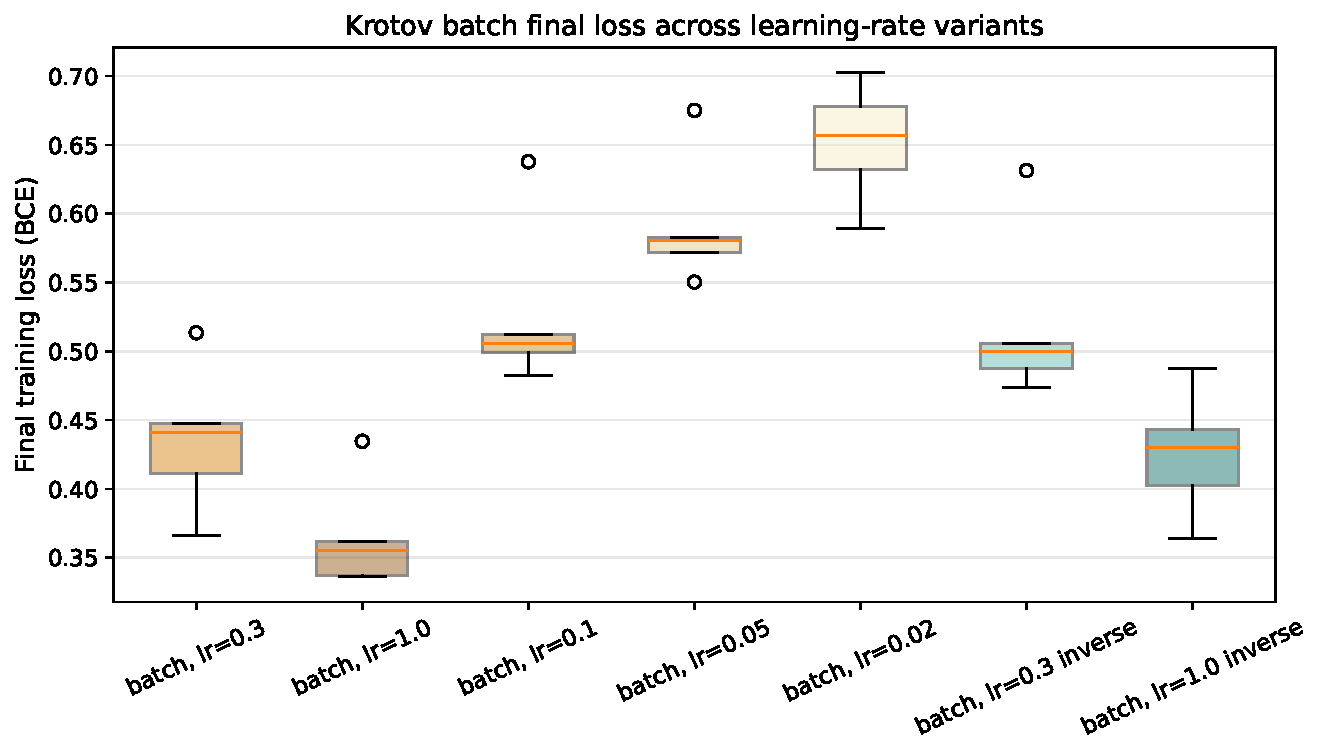
\includegraphics[width=0.92\linewidth]{figures/krotov_batch_sweep_boxplot.pdf}
\caption{Distribution of final training losses across batch-step-size variants.}
\end{figure}

\begin{figure}[H]
\centering
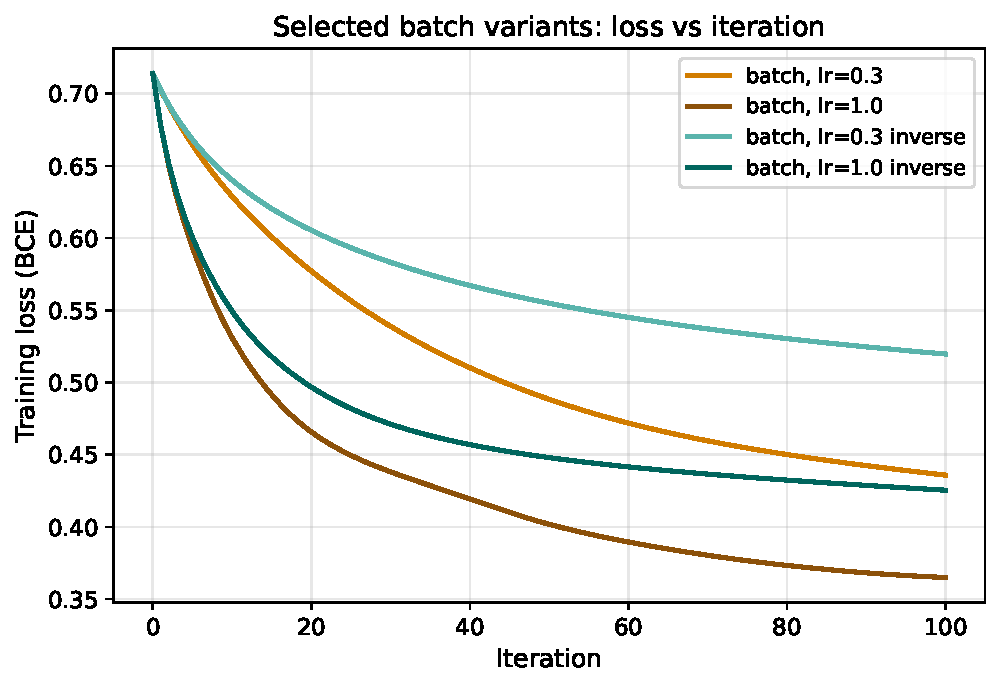
\includegraphics[width=0.82\linewidth]{figures/krotov_batch_selected_variants.pdf}
\caption{Selected batch variants. Larger initial step sizes recover much of the missing progress, while inverse decay trades speed for additional stability.}
\end{figure}

The sweep shows that the batch optimizer is not failing because of an obvious implementation bug. When the step size is increased, the batch method becomes significantly more competitive. In particular, the best-performing batch setting in this study is \texttt{batch, lr=1.0}, which reaches a mean final loss of 0.365. This is strong evidence that a large part of the apparent batch underperformance at the default setting came from step-size mismatch rather than from the BCE adjoint derivation or the fair-cost accounting.

At the same time, the sweep does \emph{not} eliminate the qualitative difference between the online and batch dynamics. The online rule remains the more aggressive optimizer in the early phase, while the batch rule remains the smoother and more predictable one. The evidence therefore supports the following interpretation:
\begin{itemize}
\item unfair accounting was \emph{not} the reason for the observed fast early drop;
\item stale adjoints and single-sample noise are plausible explanations for the online oscillation;
\item the baseline batch underperformance was strongly amplified by step-size choice;
\item after retuning, the batch rule is viable, but its behavior is closer to stable first-order descent than to the highly expressive, sample-adaptive online Krotov trajectory.
\end{itemize}

\section*{Selected batch variant versus Adam and L-BFGS-B}
For the direct baseline check, the strongest tested batch setting in this sweep, \texttt{batch, lr=1.0}, is compared against the stored Adam and L-BFGS-B runs on the same five seeds used in the variant study (0, 1, 2, 3, 4). The older baseline JSON logs do not contain the newer fair-cost trace, so the overlay below uses the common saved axes shared by all three optimizers: iteration and wall-clock time.

\begin{table}[H]
\centering
\begin{tabular}{lcccc}
\toprule
Optimizer & Final loss & Final test acc. & Wall time (s) & Total steps \\
\midrule
batch, lr=1.0 & 0.365 $\pm$ 0.036 & 0.852 $\pm$ 0.015 & 52.9 $\pm$ 0.1 & 100.0 $\pm$ 0.0 \\
Adam & 0.353 $\pm$ 0.032 & 0.863 $\pm$ 0.025 & 97.8 $\pm$ 0.6 & 100.0 $\pm$ 0.0 \\
L-BFGS-B & 0.353 $\pm$ 0.029 & 0.837 $\pm$ 0.010 & 79.2 $\pm$ 21.1 & 78.8 $\pm$ 21.5 \\
\bottomrule
\end{tabular}
\caption{Direct comparison on the aligned five-seed subset used in the Krotov-variant sweep.}
\end{table}

The direct overlay shows that the retuned batch method is \emph{close} to the gradient baselines, but not fully matched in final loss. On the aligned seeds, \texttt{batch, lr=1.0} reaches a mean final loss of 0.365 $\pm$ 0.036, versus 0.353 $\pm$ 0.032 for Adam and 0.353 $\pm$ 0.029 for L-BFGS-B. Its mean final test accuracy of 0.852 is similar to Adam's 0.863 and slightly above L-BFGS-B's 0.837. The strongest practical advantage of the batch Krotov variant is wall-clock speed: it finishes in 52.9s on average, compared with 97.8s for Adam and 79.2s for L-BFGS-B on this subset.

\begin{figure}[H]
\centering
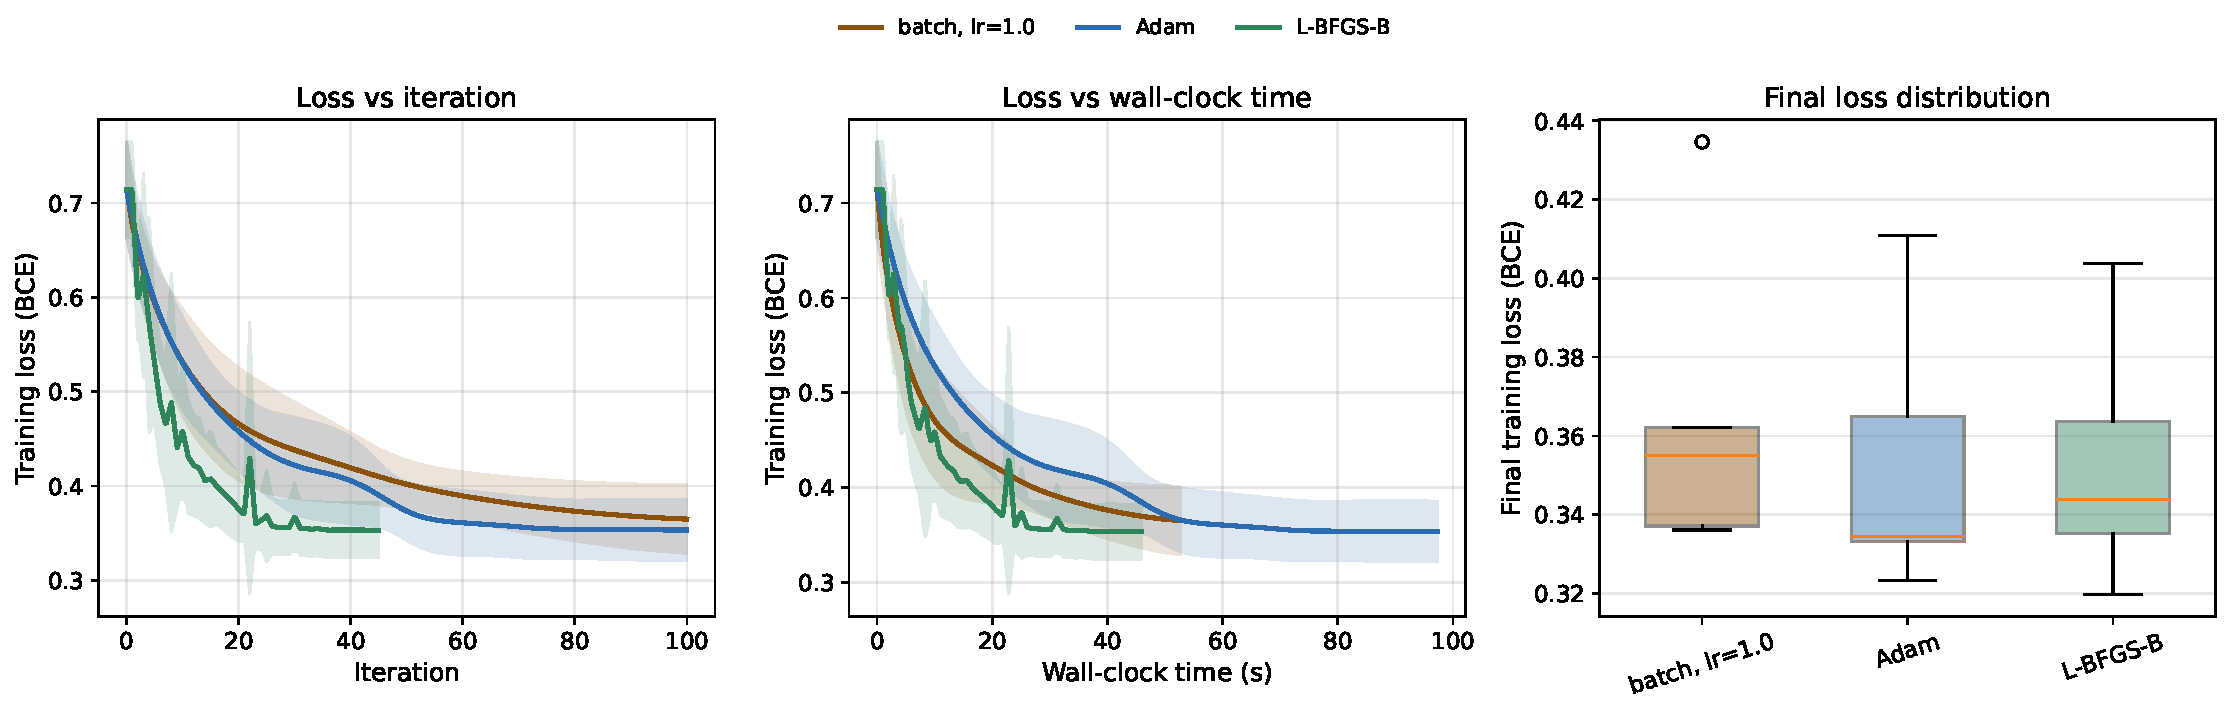
\includegraphics[width=\linewidth]{figures/selected_batch_vs_baselines.pdf}
\caption{Selected batch Krotov variant (\texttt{lr=1.0}) against Adam and L-BFGS-B. The batch method is competitive in wall-clock time and test accuracy, while Adam and L-BFGS-B still retain a small edge in final training loss.}
\end{figure}

\section*{Conclusion}
The new Krotov variants separate two effects that were previously entangled. The preserved online optimizer confirms that the original method derives real benefit from sequential sample-wise updates, but it also exhibits the largest late-stage oscillations. The new full-batch variant removes the objective mismatch and the stale-adjoint sample ordering issue, yielding a cleaner optimization signal. However, it needs a substantially larger effective step size to compete on this benchmark. The overall picture is therefore not ``implementation bug versus no bug'', but rather ``aggressive noisy online dynamics versus smoother objective-aligned batch dynamics, with learning-rate scale playing a decisive role.''

\end{document}
